\chapter{Hardware}
Un cuadricóptero o cuadrirrotor es una aeronave no tripulada (UAV) que está propulsada por cuatro motores cuyas hélices están orientadas verticalmente.Se ha diseñado y construido un cuadrirrotor casero para poder probar en la realidad el control del dron. 

Un cuadricóptero convencional cuenta con: un chasis o \textit{frame} que lo sustenta, cuatro motores y la electrónica necesaria para controlarlos, una controladora de vuelo que lo comanda y baterías que le proporcionan energía.

A continuación se detallará como són las distintas partes del dron que se ha fabricado.
\section{Cuadro}
El \textit{frame} está compuesto por perfiles de aluminio y piezas de PLA fabricadas mediante impresión 3D. Cuenta con un nivel para alojar los motores, la receptora de radio y la controladora de vuelo y otro nivel para la batería. Todas las piezas de PLA son de diseño propio y se han realizado mediante software CAD.\\


\tb{\tb{\huge imagenes modelo CAD}}.
\section{Motores y variadores(ESC)}
El dron cuenta con 4 motores sin escobillas (\textit{brushless}) LHI MT2204 II de 2300KV con una tensión de alimentación entre 7.2 V y 11.1 V (2s -3s en una batería LiPo) y una corriente continua máxima de 16A.


Estos motores son trifásicos, es decir, se alimentan con 3 corrientes alternas monofásicas de igual frecuencia y amplitud, desfasadas 120\grad \;eléctricos. Para obtener estás formas de ondas a partir de la corriente continua de las baterias, se utilizan los variadores o \textit{ESC}.\\


\newpage
\begin{figure}[htb!]
	\centering
	\begin{subfigure}{0.4\textwidth}
		\centering
		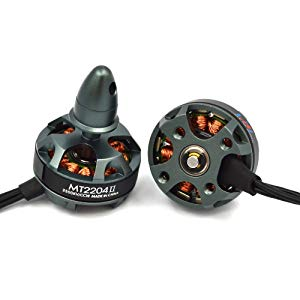
\includegraphics[width=0.8\textwidth,height=0.2\textheight]{hardware/motores.jpg}
		\caption{Motores LHI MT2204 II empleados}
		\label{hardware:motores}
	\end{subfigure}
	\begin{subfigure}{0.4\textwidth}
		\centering
		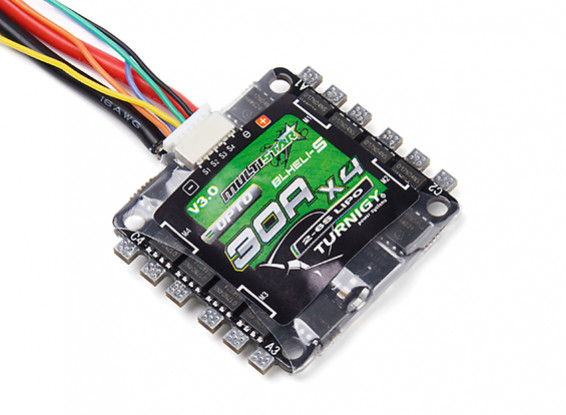
\includegraphics[width=0.8\textwidth,height=0.2\textheight]{hardware/esc.jpg}
		\caption{ESC Multistar Race 4 in 1 30A BLHeli empleado}
		\label{hardware:esc}
	\end{subfigure}
\end{figure}


Un variador o \textit{ESC (Electronic speed control)} es un circuito electrónico que controla y regula la velocidad de un motor eléctrico. \\

\tb{\Huge Profundicar en las ondas generada por el ESC}
\section{Baterias}
Para alimentar al dron, se han elegido baterias tipo LiPo por su alta tasa de descarga (la batería que se ha escogido es capaz de entregar hasta 130 A) y la su estabilidad en la tensión mientras están cargadas.


\begin{figure}[htb!]
		\centering
		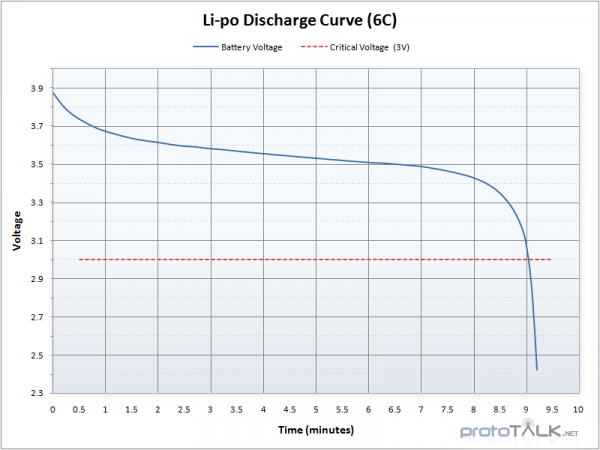
\includegraphics[width=0.8\textwidth]{hardware/curvaLipo}
		\caption{Curva típica de descarga de una bateria LiPo (fuente: ProtoTalk.net)}
		\label{hardware:curvaLipo}

\end{figure}


\section{Autopiloto}

En los drones, el sistema que se encarga de estabilizar al cuadricóptero y hacerlo pilotable se denomina la controladora de vuelo o el Autopiloto. Existe una gran variedad de controladoras en el mercado, pero para este trabajo se ha diseñado una controladora propia con el fin de poder tener acceso a todos los sensores y a implementar el algoritmo de control de forma óptima. El autopiloto consta de 3 partes diferenciadas: la electrónica de potencia, el microcontrolador y los sensores. A continuación \tb{se tratará} sobre estas partes con más detalle.\\


\tb{Estaría bien un par de imágenes de la PCB (anverso y reverso)}\\

\begin{figure}[htb!]
	\centering
	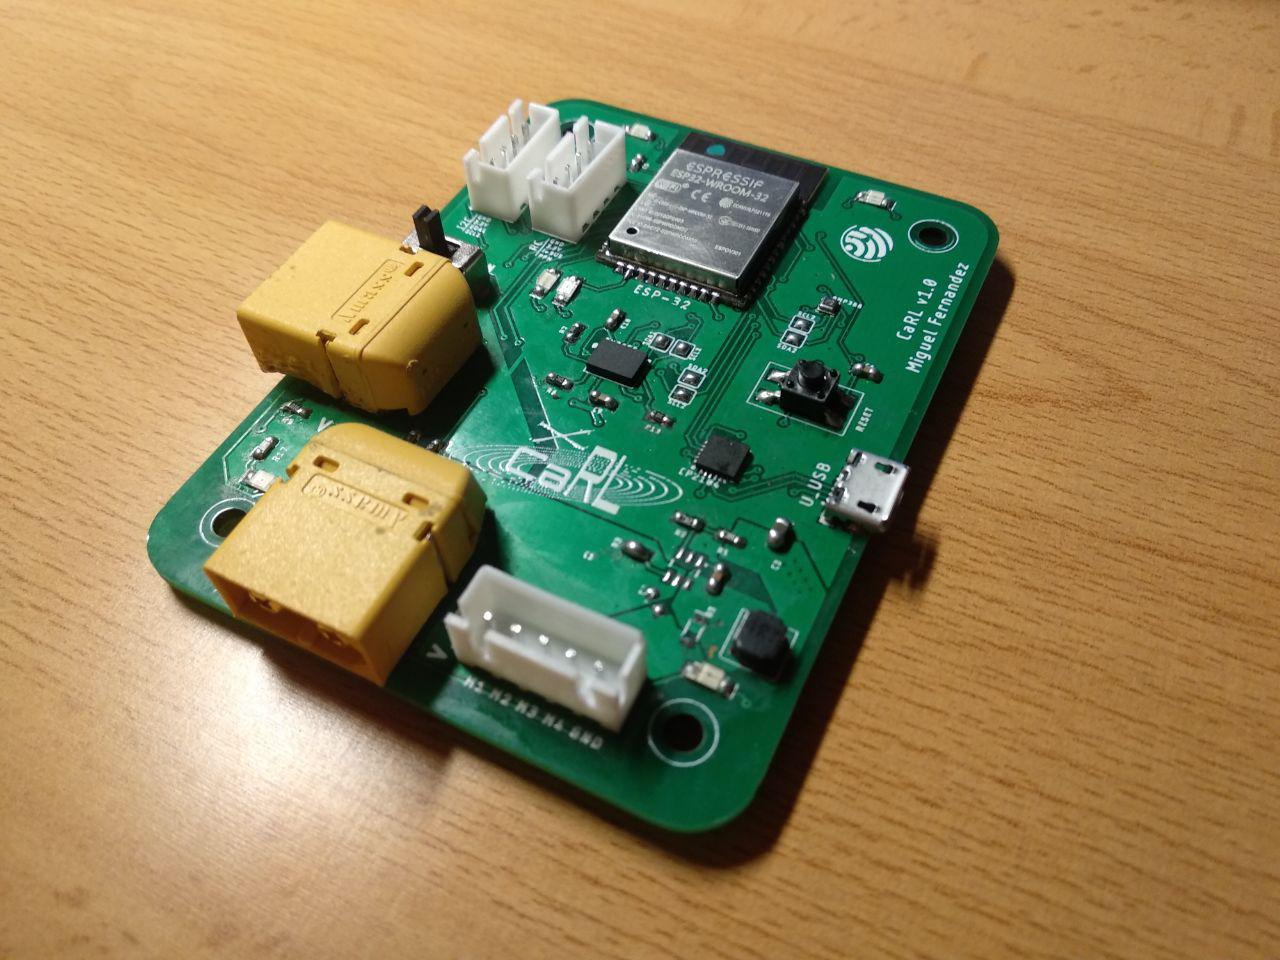
\includegraphics[width=0.8\textwidth]{hardware/carl_board}
	\caption{Autopiloto CaRL (\textit{Cuadcopter with autopilot based on Reinforcement Learning}).}
	\label{hardware:carl_board}	
\end{figure}



\subsection{Fase de Potencia}

Con el fin de poder gestionar la potencia entregada por las baterias a la placa y a los motores se ha diseñado una etapa de potencia en la que se debe mencionar dos partes: el interruptor de potencia y el regulador a 3.3 Voltios.

\subsubsection{Interruptor de potencia}

Los motores del dron pueden llegar a consumir 12 Amperios cada uno, lo que los cuatro motores pueden llegar a consumir 48 Amperios. Un interruptor con tamaño reducido no puede manejar tanta corriente, por ello se ha empleado un transistor MOSFET de canal P por el que pueden circular hasta 100 Amperios, con el fin de abrir o cerrar el paso de corriente desde las baterías al resto de la placa. El MOSFET se controla con un interruptor de poca potencia entre drenador y puerta.\\

Cuando se cierra el interruptor se alimenta directamente al ESC y al regulador de tensión.


\subsubsection{Regulador a 3.3V}

La eléctronica digital de la PCB se alimenta y emplea lógica a 3.3 Voltios, por lo que no la podemos conectar a las baterías de 11.1 Voltios.  Para adecuar la tensión se ha escogido un regulador Step-down de tipo Buck (Figura \ref{hardware:Buck}) \tb{(¿explico como funciona un convertidor Buck?)}. El circuito integrado que se encarga de conmutar la fuente es el chip AP3211.
\begin{figure}[htb!]
	\centering
		\begin{circuitikz}[american voltages,european resistors,scale=1]	
		
		\draw
		(0,2) to [V=$V_{in}$]  (0,-2)
		(0,2) to ++(1.5,0)
		++(0.5,0)node[nigfete,bodydiode,rotate=90]{}  to ++(2,0);
		
		\draw 
		(0,-2) to ++(4,0)
		++(0,0)[sD*] to ++(0,4)
		;
		\draw 
		(4,2) to [L=$L$,i=$i_L$] ++(3,0);
		\draw
		(7,2) to [C,l_=$C$] ++(0,-4)
		;
		
		\draw
		(7,2) to ++(3,0) 
		to [R =$R_{load}$,i=$i_{Load}$] ++(0,-4)
		to (0,-2)
		;
		\draw (2,0.75)node[]{\footnotesize SW};
		\draw (9.5,0.5)[short] to ++ (0,-0.5);
		\draw[-latex]
		(9.5,0)node[left] {$V_{out}$} to ++(0,-0.5);	
		
	\end{circuitikz}
	\caption{Esquema de un convertidor Buck}
	\label{hardware:Buck}
\end{figure}


\subsection{El microcontrolador (ESP32)}

El microcontrolador por el que se ha optado para este Autopiloto es el ESP32, un microcontrolador de doble núcleo con dos CPUs XTensaL6 con arquitectura Harvard \cite{ESP32TechnicalReference}. El ESP32 tiene una frecuencia de reloj de hasta 240MHz ,y cuenta con una antena WiFi a 2,4 GHz y conexión Bluetooth 4.2 BLE \cite{ESP32DataSheet}. Los motivos por los que se ha decidido emplear este microcontrolador son:
\begin{itemize}
	\item Elevada frecuencia de procesamiento y dos nucleos de procesamiento.
	\item Antena WiFi incorporada.
	\item Bajo consumo de potencia.
\end{itemize}

\par Para poder programar el microcontrolador se utiliza un convertidor USB (Bus Serie Universal) a UART (Transmisor-Receptor Asíncrono Universal) que permite conectar por USB el microcontrolador para poder programarlo y hacer depuración utilizando comunicaciones Serial. El chip que realiza esta funcion es el CP2104.

\subsection{Sensores}
La principal fuente de información procedente del exterior que recibe una controladora de vuelo se la proporcionan las unidades de medición inercial (IMU). Las IMUs son dispositivos electrónicos que son capaces de medir aceleraciones, velocidades y detectar la orientación de un sistema. El principal problema de estos sensores es que suelen sufrir error acumulativo.
\tb{¿profundizo en los sensores MEMS (imus electrónicas )?}\\


\par Otros sensores utilizados frecuentemente en los autopilotos son brújulas (se encuentran integrados en la IMU para corregir errores de orientación) y barómetros (para estimar la altitud a la que se encuentra el dron).\\
\medskip

Nuestro autopiloto cuenta con dos IMUs de 9 Grados de Libertad y un barómetro para conseguir una mejor estimación del estado del cuadricóptero:

\begin{enumerate}
	\item \textbf{BNO 055 (BOSCH)}: El circuito integrado de Bosch es un sensor "inteligente" que incluye los sensores y la fusión de las lecturas de los distintos sensores en un único componente.
	Este sensor nos proporciona estimaciones del estado con muy poca deriva. \tb {argumentar un poco mejor}
	
	\item \textbf{MPU 9250 (TDK InvenSense)}: El sensor inercial de TDK tiene una mejor respuesta dinámica, aunque la fusión de las lecturas del sensor se realiza externamente en el microcontrolador del dron.
	
	\item \textbf{BMP388 (BOSCH)}:
\end{enumerate}

%\section{Otros (Receptora radio)}

\section{Banco de pruebas}
Para poder realizar la experimentación real de forma segura, se ha diseñado una base para sujetar al drone permitiendo que rote en roll pitch y yaw de forma restringida.

La estructura de sujección esta formado por 2 juntas esféricas acopladas una a continuación de la otra, para permitir la rotación en el espacio. 
\\

\tb{\huge imagen rotulas y/o CAD }
\\

Los límites físicos de las rótulas permiten que el dron tome orientaciones comprendidas entre:
\begin{align*}
	 -60 \degree &\le \varphi \le 60\degree \quad \;\;\;  \text{Roll}\\ 
	 -60 \degree&\le \theta \le 60\degree \qquad  \text{Pitch} \\
	 -180 \degree&\le \psi \le 180\degree\quad \;  \text{Yaw}
\end{align*}

